\def\QRCODE{TB_IPR_TUT.IMG.binary_morphological_skeletonization_matlabqrcode.png}
\def\QRPAGE{http://www.iptutorials.science/tree/master/TB_IPR/TUT.IMG.binary_morphological_skeletonization/matlab}
\mcorrectionsection{Matlab correction}

\begin{mcomment}
\begin{mremark}
Please notice that when using boolean arrays in matlab, the notations \minline{1-X} and \minline{~X} are equivalent. When using \minline{uint8} arrays, verify that the values range into [0;1].
\end{mremark}
\end{mcomment}

\subsection{Hit-or-miss transform}
The hit-or-miss transform is illustrated in Fig.\ref{fig:morphological_skeleton:matlab:hitormiss}. 
\begin{figure}[htbp]
 \centering
 \subfloat[Original image.]{
\includegraphics[width=4cm]{mickey.png}\label{fig:morphological_skeleton:matlab:hitormiss:mickey}}\hspace*{1cm}
 \subfloat[Hit or miss result (intensities are inverted).]{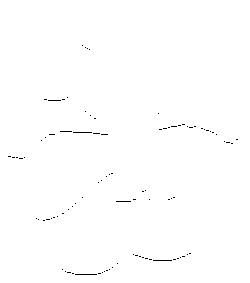
\includegraphics[width=4cm]{hitormiss.png}\label{fig:morphological_skeleton:matlab:hitormiss:result}}
 
 \caption{Hit or miss illustration for a given orientation.}
 \label{fig:morphological_skeleton:matlab:hitormiss}
\end{figure}
\begin{matlab}
function B=hitormiss(X,T)
% X is the binary image (values 0 or 1)
% T is the structuring element

T1=(T == 1);
T2=(T == -1);
B=min(imerode(X,T1),imerode(~X,T2));
\end{matlab}

\subsection{Thinning and thickening}
Thinning and thickening are dual operations. The second function could make a call to the first one. The code elementary follows 
the definition. The illustration is presented in Fig.\ref{fig:morphological_skeleton:matlab:thinning}.

\begin{matlab}
function B=elementary_thinning(X,T)
% thinning function
% X: binary image
% T: structuring element
B=X-hitormiss(X,T);
\end{matlab}

\begin{matlab}
function B=elementary_thickening(X,T)
% thickening function
% X: binary image
% T: structuring element
B = min(X, ~hitormiss(X,T));
% equivalent notation:
% B = X-hitormiss(X,T);
\end{matlab}

\begin{figure}[htbp]
 \centering
 
 \subfloat[Thinning.]{
\includegraphics[width=4cm]{thinning.png}\label{fig:morphological_skeleton:matlab:thinning:thinning}}\hspace*{1cm}
 \subfloat[Thickening.]{
\includegraphics[width=4cm]{thickening.png}\label{fig:morphological_skeleton:matlab:thinning:thickening}}
 
 \caption{Thinning and thickening.}
 \label{fig:morphological_skeleton:matlab:thinning}
\end{figure}

\subsection{Skeletons}
The pairs of structuring elements are defined like this, in the 8 directions:
\begin{matlab}
TT=cell(1,8);
TT{1}=[-1,-1,-1;0,1,0;1,1,1];
TT{2}=[0,-1,-1;1,1,-1;0,1,0];
TT{3}=[1,0,-1;1,1,-1;1,0,-1];
TT{4}=[0,1,0;1,1,-1;0,-1,-1];
TT{5}=[1,1,1;0,1,0;-1,-1,-1];
TT{6}=[0,1,0;-1,1,1;-1,-1,0];
TT{7}=[-1,0,1;-1,1,1;-1,0,1];
TT{8}=[-1,-1,0;-1,1,1;0,1,0];
\end{matlab}

Thus, the thinning operation is coded as:
\begin{matlab}
function B=thinning(A,TT)
B=A;
for i=1:length(TT)
    B=B-hitormiss(B,TT{i});
end
\end{matlab}

The topological skeleton is the iteration of the thinning with structuring elements in all 8 directions. It has the property of preserving the topology of the discrete structures, contrary to the morphological skeleton (see Fig.\ref{fig:morphological_skeleton:matlab:skeletons}.
The morphological skeleton does not preserve the connexity of the branches, but it can be used to reconstruct the original image. Pay attention to the construction of structuring elements, which should be homothetic ($B_r=\underbrace {B_1\oplus \cdots \oplus B_1}_{{r{\mbox{ times}}}}$).
\begin{matlab}
% topological skeleton function
% X: binary image
% T: structuring element
function B=topological_skeleton(X,TT)
B2=X;
B=~B2;
while (isequal(B,B2)~=1)
    B=B2;
    B2=thinning(B,T);
end
\end{matlab}


\begin{matlab}
function S=morphological_skeleton(X)
% morphological skeleton function
% X: binary image
S=zeros(size(X));
strel_size=0; % size of structuring element
pred=true;
while pred
    strel_size=strel_size+1;
    E=imerode(X,strel('disk',strel_size));
    if sum(E(:))==0
        pred=false;
    end
    S=max(S,E-imopen(E,strel('disk',1))); 
end
\end{matlab}


\begin{figure}[htbp]
 \centering
 \subfloat[Topological skeleton.]{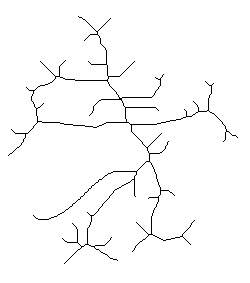
\includegraphics[width=5cm]{topological_skeleton.png}\label{fig:morphological_skeleton:matlab:skeletons:topological_skeleton}}\hspace*{1cm}
 \subfloat[Morphological skeleton.]{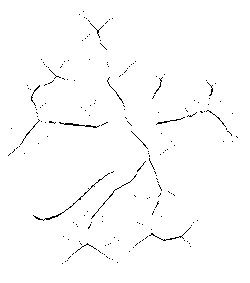
\includegraphics[width=5cm]{morphological_skeleton.png}\label{fig:morphological_skeleton:matlab:skeletons:morphological_skeleton}}
 \caption{Skeletons. The topology is not preserved in the morphological skeleton, but it can be used to reconstruct the original image. The intensities are inverted in order to facilitate the display.}
 \label{fig:morphological_skeleton:matlab:skeletons}
\end{figure}

